% !TeX spellcheck = en_GB
\documentclass[a4paper,11pt,notitlepage]{article}
\include{structure}
\hyphenation{Some-long-word}
\usepackage{amsmath}
\usepackage{fullpage}
\usepackage{graphicx}
\usepackage[english]{babel}
\usepackage{float}
\usepackage{listings}
\usepackage{color,soul}
\usepackage{pdflscape}
\usepackage[hyphenbreaks]{breakurl}
\usepackage[hyphens]{url}
\usepackage[margin=1cm]{caption}
\usepackage{subcaption}

% Title Page
\title{Laughter Detection using Neural Networks}
\author{John Scolaro\\
	Supervisor: Scott Heath\\
	Janet Wiles}

\begin{document}
%\maketitle
\thispagestyle{empty}
\begin{center}
	\begin{minipage}{0.75\linewidth}
		\centering
		%University logo
		
\includegraphics[scale=0.25]{figs/logo.jpg}
		\par
		\vspace{3cm}
		%Thesis title
		{\uppercase{laughter detector\par}}
		\vspace{3cm}
		%Author's name
		{\Large Author: John Scolaro\par}
		{\Large Supervisors: Scott Heath\\Janet Wiles\par}
		\vspace{3cm}
		%Degree
		{\Large Thesis Report\par}
		\vspace{3cm}
		%Date
		{\Large October 2016}
	\end{minipage}
\end{center}

\addcontentsline{toc}{section}{Title Page}

\clearpage

\addcontentsline{toc}{section}{Abstract}

\null\vspace{\fill}
\begin{abstract}
	This thesis proposes a new way of detecting laughter using neural networks. It detects laughter on a frame-by-frame level, allowing it to estimate when laughter starts and stops which contrasts to older methods of laughter detection which classify a chunk of audio all at once. Several different methods are tried and tested, with the results presented here, with a simple feed forward neural network achieving the greatest accuracy when trained on sequences of MFCC's from audio.
\end{abstract}
\vspace{\fill}

\clearpage

\addcontentsline{toc}{section}{Table of Contents}
\renewcommand*\contentsname{Table of Contents}

\tableofcontents

\clearpage

\section{Introduction}

% Basically a quick introduction skimming over all the topics covered in the whole report.
	% What I'm doing
	% Why it's a neat idea
	% What there already is
	% How I'm improving it
	% What the results were super briefly

This report discusses the results obtained by attempting to detect spontaneous human laughter in audio with neural networks. In the process of doing this, many choices were made in all aspects of the design of this project, and this report will attempt to explain all of them in as much detail as possible - starting with the collecting of audio to create a dataset of speech and laughter, and ending with the creation of different networks and a discussion of their results.

\subsection{Motivation}

% Why I am trying to do it

Extracting information from audio has many uses, including speech recognition and song detection, which many people use every day. In audio recordings of human speech, more information is present than just the spoken words. Humans can glean information from the speaker, from the speed at which they talk, the tone and volume used,\cite{dellaert1996recognizing} or perhaps the amount of fillers, `umming' and `ahhhing', between sentences.\cite{brennan1995feeling} In the book ``Silent Messages''\cite{mehrabian1971silent} the author A. Mehrabian talks about his work on non-verbal communication. He concludes that listeners assign 55\% of their attention to the speakers stance and body movements, 7\% on the words they say, and 38\% on the way they say them. The mood of the speaker gives further information about what their words mean, and how they feel. Being able to detect these various audio cues allows for better interpretation of the sentiments underlying human speech. Examples of systems which utilise these additional audio features include anger detection, which could be implemented in call centres to route frustrated callers directly to humans operators,\cite{yacoub2003recognition} or the detection of applause, which can be used to segment video and summarize large events.\cite{cai2003highlight} One of the most prominent non-verbal features of human speech is laughter as it gives information about the mood of the laugher and can be associated with several emotions. State-of-the-art speech detection systems are approaching 100\% accuracy at determining exactly what is being said, but detecting laughter is one of the first of many steps to attempt to decode the context in which it is being said.\\
\\
Laughter is often a loud and repetitive sound, and similarly to speech, easily detectable by a human listener. However due to the complexity of the sound, it is difficult to precisely classify computationally. These types of problems are perfect for machine learning. Questions which can be answered by any human, but when asked how, it isn't really explainable. ``How can you tell there is a face in that picture?'' or ``What words are being said in this audio?'' are other examples. As a human, you just can. There is no simple mathematical expression you can write to distinguish exactly what is in a picture based on the pixels, but if you look at the picture, you can simply see what is there. There are many types of laughter, which can be categorized a number of ways. For example, a simple classifier separates laughter into voiced and unvoiced categories, where voiced laughter is louder and song like, while unvoiced laughter consists of grunts and snorts. Additionally, laughter is used differently in different scenarios to mean various things: from softer polite laughs, to louder more jovial laughs used amongst friends.\cite{tanaka2011acoustic} Laughter also changes in the company of people of different gender and nationality,\cite{campbell2007whom} and affects the opinions of people listening.\cite{bachorowski2001not} Accurate laughter detection has many practical applications. These applications include but are not limited to: the detection of humorous content, improvement of speech recognition software by recognising non-speech sounds, and facilitating more natural machine-human communication. Previous studies can be divided into those which attempt to detect laughter in audio, and those which attempt to classify the type of laughter. The best laughter detectors use standard speech recognition features and discriminating techniques\cite{cosentino2016quantitative}, with some of the best classifiers achieving ~10\% error.\cite{gosztolya2016laughter,knox2007automatic,truong2007automatic,truong2005automatic} Extending on laughter detection, laughter classification allows further unvoiced information to be extracted from audio about the type of laughter. Knowing whether laughter is uncomfortable or genuine can be used to improve machine-human interaction. Laughter classification has been shown to work successfully using Hidden Markov Models (HMM) on standard audio features\cite{tanaka2011acoustic}, however this research was only tested with a training set of ~150 laughter segments, so it is far from comprehensive.\\
\\
At the University of Queensland, this project is of interest to two different research groups. The linguistics department who hopes to learn more about the general structure of laughter and different types of laughter, and the Complex \& Intelligent Systems Research Division, which is both interested in laughter and it's detection for interaction with humans, and the neural networks behind its detection.\\
\\
+Curiosity\\
\\
+Laughter classification is potentially useful for a large number of reasons.\\
\\
+Nobody else has done it this particular way before.

\subsection{Aim}

% What it is that I'm trying to do

The aim of this thesis is to design a neural network to detect laughter as accurately as possible. Through designing and testing many different neural network architectures some intuition can be gained as to how the node weights change to detect laughter. Different audio features may be of different importance, and the change in features' weights over time may also give information about the average laughter sound. In essence, one main goal is to derive some intuition about fundamental differences between laughter and speech, which allow the network to discriminate between them.\\
\\
The neural network this study aims to create will classify sequences, rather than short clips of audio which is a slight difference to other research into laughter detection. [INSERT REFERENCE] The aim is to be able to process any arbitrary length audio sample or file, and the program will return the probability of the audio being laughter at every point of the file. This contrasts work by [INSERT REFERENCE] who created a system for discriminating between small sections of audio by determining if they contained laughter in them. If the rough start and end times of laughter can be determined in any audio file, that represents a much finer and more accurate laughter detection system.\\
\\
Another goal of this study is to replicate similar\cite{gosztolya2016laughter} recent works on laughter detection, and potentially extend upon them. These recent works use deep neural networks to classify laughter, which can be implemented in TensorFlow. More recently Long Short Term Memory (LSTM) networks have achieved more accurate results on problems with sequential data, like human speech.\cite{hannun2014deep,mozilladeepspeech} TensorFlow provides high level tools to create an LSTM network which may allow for this to be investigated within the time-frame of this thesis.

\newpage

\section{Background}

% An in depth look into the state of the field of study so far

The study of laughter detection uses knowledge from a number of different fields. Laughter detection looks to studies in the field of linguistics for information about phonetics and how sounds like laughter and speech are generated. For the detection, recent advances in the fields of machine learning for speech recognition are used. All these niche fields draw on findings from fields such as: transcription, signal processing, sequence detection, neural networks and computer science. In this background section, a more detailed look with be taken into the outcomes of previous laughter detection studies, different signal processing and machine learning techniques, and other studies from areas influencing this report. 

\subsection{Laughter}\label{subsection:laughter}

% This section will talk about the study of laughter from a linguistics point of view. The phonetics, stats, emotions, other stuff like that.

Laughter is a complex signal. There are many different ways to approach the issue of characterising laughter, and many different researchers have conducted research analysing laughter approaching it from many different directions. Laughter can be looked at from an emotional perspective, examining the way it makes the listened feel. It can be studied from a purely linguistic and biological perspective, analysing the mouth and throat movements responsible for creating it. Studies have been conducted examining how patients change their laughter depending on who they are talking to, or where they came from. Laughter can also be phonetically analysed in the same way as speech, categorising the different laughter `syllables' in the same way syllables in speech are categorised.\\
\\
% General laughter
A rigorous study into laughter was conducted by Bachorowski in 2001\cite{bachorowski2001acoustic} on the acoustics of human laughter. Just over one thousand laughter segments were classified and analysed from recordings taken from willing students. The laughter was collected by recording ninty-seven students watch humorous clips from movies, and recording their responses. Laughter was analysed at `bout', `call', and `segment' levels. Here, bouts refer to an entire laughter episode occurring during a single exhalation, and although these frequently end with a sharp inhalation, this was not classified as part of the laughter. Calls refer to the individual `laughter-syllables' within the bout, and segments are sections within a call where a change in frequency occurs. Several large and interesting laughter statistics were noted from this study, such as laughter sex not affecting the number of laughs produced and females producing more song-like laughter bouts while males produced more unvoiced grunt-like laughs. It also collates the findings of seven other papers investigating laughter, and compares several laughter features (laughter stimulus, number of laugh bouts, calls per bout, bout duration, and more) all recorded by each of the papers and compares them to each other. This paper makes four conclusions, of which the first and most prominent is that ``Laughter is highly variable''. It seems depending on the subject, the method of obtaining laughter, and many other factors, the statistics gathered about the laughter seem to vary greatly. This paper breaks laughter into three different categories: song-like, grunt-like, and snort-like. Song-like laughs are more stereotypical laughs which would be described as `giggles' and `chuckles'. They consist of small, repetitive voiced sounds. Snort-like laughs were described as: ``Bouts largely comprised of unvoiced calls with perceptually salient nasal-cavity turbulence'', and grunt-like laughs as breathy pants caused by turbulence from either the laryngeal or oral cavities.\cite{bachorowski2001acoustic}\\
\\
% Classifications of laughter
\subsubsection{Laughter Classification}
On the subject of laughter classification, most papers separate laughter into a variable number of categories for the purpose of their investigation. As mentioned previously, Bachorowski identified three different laughter types, song-like, grunt-like, and snort-like. Different papers separate laughter into different categories, for example Hiroki Tanaka's paper: ``Acoustic Features of Four Types of Laughter in Natural Conversational Speech''.\cite{tanaka2011acoustic} Tanaka notes that previous research revealed that while ``Laugher played an important role in all dialogues but the laughs only occasionally resulted from deliberate humour; polite laughter and nervous social laughter accounted for more than half the number of laugh bouts''\cite{campbell2007changes}. In Tanaka's own study, laughter was classified into one of five different groups: mirthful, polite, embarrassment, derision, and other, separating laughter into classes by its social use, rather than it's formation. The paper then goes on to show the differences between each of these types of laughter.\\
\\
\begin{figure}[H]
	\centering
	\vspace{0.5cm}
	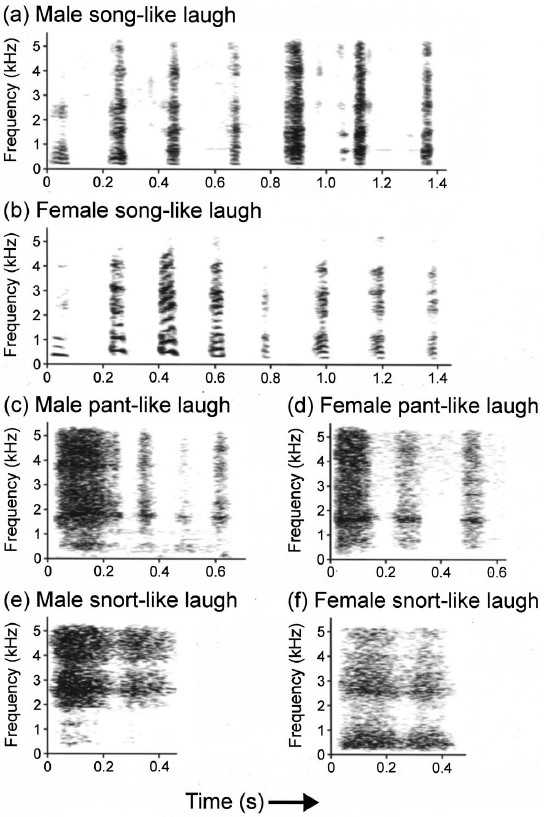
\includegraphics[scale = 0.5]{figs/laugh_spectrogram_from_bachorowski.png}
	\caption{Spectrogram visualisations of laughter from each of the tree different classifications in Bachorowski's paper. The difference in frequency structure of each laugh is easily seen, with harmonics in song-like laughter much more apparent.\cite{bachorowski2001acoustic}.}
	\label{laughter_spectrogram_from_bachorowski}
\end{figure}
% Different situations when laughter is different.
Laughter also changes when produced under different circumstances. In N. Campbell's paper: ``Whom we laugh with affects how we laugh''\cite{campbell2007whom} a neural network is created and training on a single persons laughter when talking to a range of different people. The network learns to discriminate (with an accuracy slightly below 50\%) between with whom the speaker is speaking purely by the difference in laughs they make, proving that there is some difference in laughter features in different situations. This paper focussed on the differences in laughter when talking to people of different gender and of different ethnicity.\\
\\
% Biological laughter production
\subsubsection{Laughter Production}
% Laughter averages, ie frequency, length, call number, all that.
Laughter is a complex physical response, involving many different sections of the body. A number of studies look at the different bodily actions that occur during laughter. These responses can be seperated into five different areas:\cite{cosentino2016quantitative}
\begin{itemize}
\item Acoustics (The emitted sound)
\item Respiration
\item Phonation (The audio features, or shaping, of the emitted sound)
\item Facial Expression
\item Whole body movement
\end{itemize}
Recently a number of studies attempt to detect laughter by analysing a number of these different modes of expression simultaneously.\cite{petridis2008audiovisual,scherer2009multimodal} From an acoustical standpoint, laughter has several easily measurable features. These have been measured in many different studies, but averages for each of them have been found in a paper summarising hundreds of papers studying laughter written by S. Consentino\cite{cosentino2016quantitative}, and these are the numbers quoted below. A typical mirthful laugh contains four or five calls, and the average length of a call is about 220ms. Earlier calls tend to be louder than later ones, most likely due to a decreasing air supply. For both male and female laughter, the typical fundamental frequency is approximately 20\% higher pitch than in casual speech at ~278Hz for males, and ~480Hz for females. Voiced pulses may contain audio at a frequency higher than 16kHz, but most power is contained below 8kHz. The precise phonation of laughter has been measured precisely by using invasive intramuscular electromyogram signals.\footnote{These studies placed bands around the abdomen and chest of the patients and up to four small electrodes were injected into different laryngeal muscles. Despite having many electrodes embedded in their throats, the patients were all able to speak, swallow, and laugh comfortably.} Very complex analysis has been done on these detailed tests, revealing precisely how all the different muscles in the throat and neck move during laughter. Such descriptions are heavily biological, for example: ``During adduction, the thyroarytenoid and the cricothyroid muscles close the glottis, the arythenoids approach each other at a constant rate, and the vocal folds start vibrating while they are still not fully closed. Instead, during abduction, the posterior cricoarytenoid muscle is responsible for the opening, and the vocal folds are still vibrating when the abduction phase begins.''\cite{cosentino2016quantitative}\\
\\
While the precise movements of all the larynx and throat tissues isn't exactly required to develop a laughter detector, it is important to note the complexity of the structure of laughter, and the many different contributing factors which go into the creation of its sound. Analysis into the cause of differing laughter pitch alone is complex: ``Changes in the fundamental frequency F0 might be determined by multiple factors: the shortening of vocal tract length, due to lowering or lifting of the larynx, or to protraction or retraction of the lips, the tension and lengthening of vocal cords, and the variation of tracheal pressure which can, but not always, be temporally correlated with laryngeal adductors.''\cite{cosentino2016quantitative} It is this complexity to laughter which makes creating a laughter detector utilising purely phonetic theory such a hard task. Indeed, when talking about the different factors which make up laughter, Fry and Rader state: ``The interaction of these factors generates an almost infinite number of individually different laughs.''\cite{fry1977respiratory}

\subsubsection{The Social Role of Laughter}
% Laughter as it relates to social interaction.
% Social standings and heirachy.
Laughter is most often induced by something funny, and is a powerful conveyor of information. Laughter shows involvement in conversation and lets other people know that you have found something humerus. Besides this most common form of laughter, it can also be used to express other emotions such as stress and frustration. Another interesting observation is that people laugh more often when people around them are laughing. This is why laughter is often said to be `contagious'. This may be why the first comedian at a comedy club is tasked with `warming up the crowd', and laugh-tracks in sit-coms are employed to make a show seem more entertaining.\\
\\
% Simply as a sound
The interactions between laughter and speech are quite interesting. In a polite conversation between two people, most often only a single person is talking at one time and interruptions are kept to a minimum. Laughter is the opposite and if someone laughs, it is socially acceptable to laugh at the same time, and often politeness brings us to laugh when someone else does, even if we do not find anything particularly funny.\cite{dupont2014acoustic}\\
\\
% Power
As previously mentioned in subsection \ref{subsection:laughter}, laughter is used very differently depending on the social situation it is used in. One area of study in this field is the use of laughter in different power dynamics. In a paper by C. Rees, she looks in detail at a number of conversations which occur in a patient-doctor-student situation at a doctors office. In these scenarios there is a doctor and a student working directly under the doctor consulting a patient. The role of power in the workplace is looked at through the use of laughter by all parties. She concludes that: ``The laughables can be construed as teases of various kinds: fallibility, frustration, cynicism and/or sexual teasing. Although some of the teases may have been attempts by participants to construct intimacy, we believe that the teases functioned primarily to construct power, identity and gender.''\cite{rees2010should} In another paper looking at laughter in social work, it is noted that there is much more laughter between the social workers than there is between their clients. It is concluded that laugher is used: ``(Laughter is) employed by staff members as: (1) a way to create informal settings between staff and clients; (2) a way to deal with situational tensions/ambiguity in the work; and, (3) a way to deal with organizational contradictions in working with clients.''\cite{mik2007interpersonal}\\
\\
In a study by J. Bachorowski, students at a university listened to different recorded laughter segments for several people, and told to rate each subject in terms of `how interested to meet them' they would be. They found that both males and females are much more interested in meeting someone who uses voiced laughter more often than unvoiced grunts, pants, and snortlike sounds.\cite{bachorowski2001not}\\
\\
Highlighted by these studies is the large amount of depth for the different uses of laughter in social situations. This again draws attention to the large variety of different laughter types used in common situations, and the difficulty of laughter detection.

\subsubsection{Health Perspective}
% Laughter from a health perspectivex
idk if this is even worth talking about given the small amount of research done here, and how hand-wavey it is.

% Laughter synthesis
\subsubsection{Laughter Synthesis}
\cite{dupont2014acoustic}

\subsection{Datasets}

% Talk about the datasets used in other papers, and how these differ from ours, and how the results will be impacted by this.
One of the most important aspects of any machine learning problem is the procurement of a good quality dataset to train a model on. Several databases with pre-labelled laughter exist, and this section aims to analyse these databases in terms of their effectiveness in training a laughter classifier. 
\cite{dupont2014acoustic}

\subsection{Preprocessing}

% There is definately much more you can write on MFCC's here.
	% Comparison to PLP's
	% Why did you choose MFCC's?
	% How exactly do MFCC's work?
		% Plus pictures.
	% Frame size and stride.
		% Plus picture.
	% Delta's and delta deltas

\subsection{Machine Learning Techniques}

% Machine learning overview
% Statistical models
	% Markov models, and all other models used in previous papers.
	% Neural networks
	% Sequential Neural Network
	% lstm networks
	% Wavenet?

\subsection{Previous Laughter Detection Attempts}

% In this section we will talk about other laughter detection papers.
% Definately discuss the metrics they use to talk about accuracy at some point.

For example, in a study by S. Sherer, both audio, and tracked facial position were used as inputs to a laughter detector.\cite{scherer2009multimodal} In another study by S. Petridis, facial expression was broken down into four main features and used alongside audio features to aid laughter detection.\cite{petridis2008audiovisual}

\section{Methodology}

% How I've gone about my work. So this is the major heading talking about what I've done to attempt to detect laughter.
% I am unsure about whether to actually put any writing about anything in this section, or just put it all into the subsections.

When this project was started, there was no dataset or prior work on this topic, so everything from dataset procuring to network design was created for this project. This section details all the steps that were taken for each fundamental part of this project.

\subsection{Dataset}

% Starting with all my working into the dataset.
	% Talk about the audio of the dataset first.
		% How it was recorded
		% When
		% What it was for
		% The type and quality of audio
		% General statistics about the laughter.
		% Compare my dataset to other datasets and talk about the differences.
	% Preprocessing of the dataset. Removing noise. Normalizing volume roughly.
	% Talk about classification of laughter
		% My classification.
		% Compared to other peoples classification and maybe error analysis.

The dataset used for this project was a collection of recorded spontaneous speech from the Australian National Corpus. A total of eighty-one different audio clips was used, for a total audio length of fifteen hours and twenty-six minutes. These audio snippets contained conversations from students in the school yard, interview type scenarios, casual around-the-house conversation, and a variety of people in different scenarios. A majority of the recordings were taken over twenty years ago on cassette tape, and have been since converted to digital format. Conversations most frequently occur between two or sometimes three people, with the occasional recording containing more. This is important to note, as this thesis details the detection of laughter by one person, and not the detection of laughter of many people at once, as is done in other papers.\cite{kennedy2004laughter}\\
\\
This corpus is smaller than the datasets used in other studies, which have used hundreds of hours of audio from recorded meetings, or telephone calls. It is well known that machine learning techniques improve where there is more data, and with only fifteen hours of audio, our results will be limited. The laughter in the audio used in this study is very diverse, with many different types of laughs. There are long belly laughs from old friends, and very short polite laughs from a child addressing their parents. There are laughs from people with thick accents, and laughs emitted which trying to talk. The diversity of the dataset used is an advantage, as any patterns learnt should be to the nature of laughter 'in-general' and not overgeneralise to a specific type of laughter, or the laughter of one person.\\
\\
All audio files are purely recordings of human speech, and do not contain noises from other sources. Other laughter classifiers [INSERT REFERENCE HERE] have trained systems to detect laughter by using a myriad of different sounds to train on. [INSERT REFERENCE HERE] Detecting the difference between laughter and human speech will be more difficult, but potentially more useful as laughter is often interwoven between snippets of human speech, and not between the sounds of trains, popping bubbles, and waterfalls.

\subsubsection{Classification}

Prior to this study, the audio from the Australian National Corpus had never been used for laughter detection, and the data labels did not exist. Past research into laughter detection used the laughter labels that meeting transcribers had attached to the transcriptions of meetings. [INSERT REFERENCE HERE] and researchers had fiddled with portions of the data themselves because they found the data labels inaccurate. [FIND REFERENCE HERE AND MAYBE QUOTE]. However, with hundreds of hours of audio, sifting through it all manually to select the laughter would be infeasible. In this study, the audio was listened to, and the laughter segments were manually selected down to the millisecond.\\
\\
The method used to classify the laughter, was to use ELAN\footnote{ELAN is a product of the Max Planck Institute for Psycholinguistics, The Language Archive, Nijmegen, The Netherlands. It is free, and can be found here: \url{http://tla.mpi.nl/tools/tla-tools/elan/}}\cite{sloetjes2008annotation}, an audio-visual transcription software, to select the sections of audio which contain laughter. ELAN outputs this data in an XML format, which is parsed into a list of times when laughter starts, and then subsequently stops. These lists of start and stop times are used when creating the dataset, and the label (in one-hot encoded form) is appended to the vector of audio features. This list of start and stop times can also be quickly analysed to give some insight into the frequency and average laughter length in the collected dataset. The average laughter time of roughly one second in Table \ref{laughter_stats_table} agrees with findings from previous studies about the nature of laughter.\cite{bachorowski2001acoustic}\\
\\ 
\begin{table}[]
\centering
\begin{tabular}{|l|l|}
\hline
Total Laugh Count                     & 1456           \\ \hline
Total Length of Laughter              & 1480.1 seconds \\ \hline
Longest Laugh                         & 6.32 seconds   \\ \hline
Average Laugh Length                  & 1.01 seconds   \\ \hline
Audio File with Least Laughs Contains & 0 laughs       \\ \hline
Audio File with Most Laughs Contains  & 102 laughs     \\ \hline
\end{tabular}
\caption{A table containing statistics of the laughter classified in the complete dataset.}
\label{laughter_stats_table}
\end{table}
\begin{figure}[H]
	\centering
	\vspace{0.5cm}
	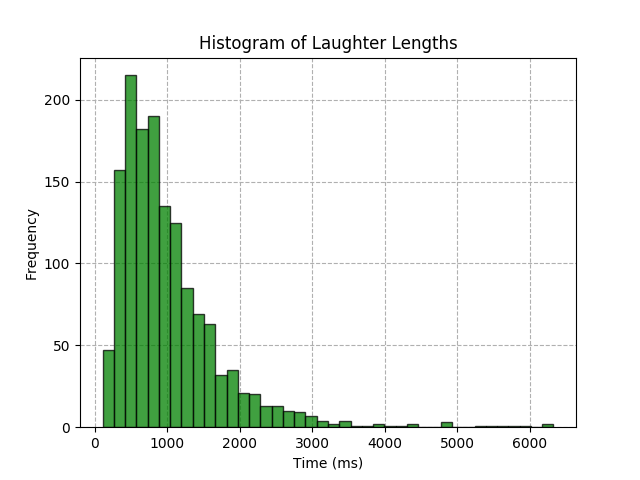
\includegraphics[scale = 0.8]{figs/laughter_length_histogram.png}
	\caption{A histogram of the laughter segment lengths.}
	\label{laughter_length_histogram}
\end{figure}
Laughter in speech is a hard audio signal to classify. It often does not have a definite start or end point. Commonly an individual laugh will be preceded by a sharp inhalation, and/or followed by a brief `ahh' sound, and every laugh is different. Some might be very quiet snickers, snorts, or just fast exhalations. What do we empirically classify as `laughter'? Rather than define `laughter' as a specific type of laughter, potentially an easily distinguishable laughter like a belly-laugh, which would make the job of classification much easier, the data was classified as what the author `felt' was laughter. In order to train a model to predict laughter as accurately as a human, it needs a human-like classification. This makes this section particularly tough to write as scientists don't enjoy saying: ``This particular section of audio `felt' like laughter'', but would rather employ some quantitative analysis to say: ''This audio is definitely laughter because...''. When it comes to machine learning with audio, we want to give the model something a human thinks is correct, and let the machine find the complex mathematical relationships which separate laughter from non-laughter. This means that while previous papers have, for example not classified the exhalation after the laugh as laughter\cite{bachorowski2001acoustic}, this report may have, so slightly different finding with respect laughter lengths are expected. \\
\\
Nevertheless, when classifying laughter, what one person `feels' is laughter, may not be identical to the observations of another person, and this is something worth investigating. In an effort to investigate differences in laughter classification between different people, two people were taught how to classify laughter using ELAN, and given a 45 minute audio clip to classify.\\
\\
In this 45 minute clip, one classifier found 87 laughter instances, and the other found 61. The actual classifications were very similar however. The main differences are that one classifier often split longer laughter segments up into multiple pieces, and included segments of laughter interwoven with speech. Example plots of the difference classifications are shown in Figure \ref{laughter_classification_differences_1} and Figure \ref{laughter_classification_differences_2}. With more classifiers, the jerky transition between laughter and non-laughter will be smoothed. Even without more classifiers, a linear interpolation method could be employed to further smooth this transition.
\begin{figure}[H]
	\centering
	\vspace{0.5cm}
	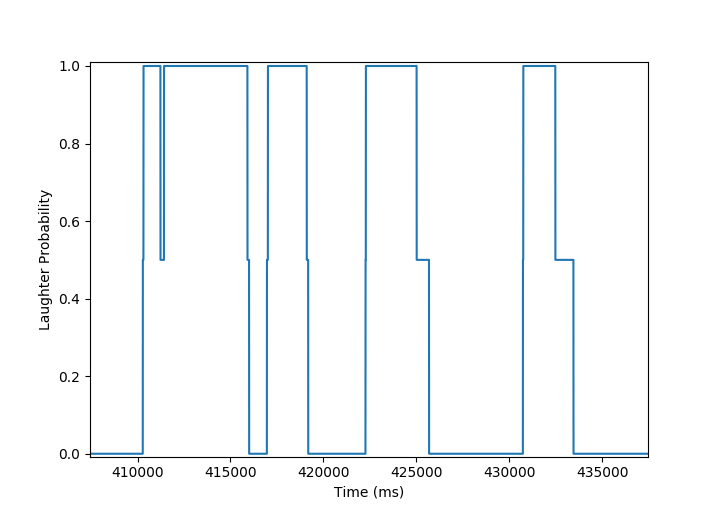
\includegraphics[scale = 0.75]{figs/differences_1.png}
	\caption{The differences in laughter classification between two different humans. Here, we see the differences in classification clearly. One classifier appears to think that laughter lasts approximately a whole second longer for the second two laughter instances, while one classifier separates the first laughter instance into two separate pieces.}
	\label{laughter_classification_differences_1}
\end{figure}
\begin{figure}[H]
	\centering
	\vspace{0.5cm}
	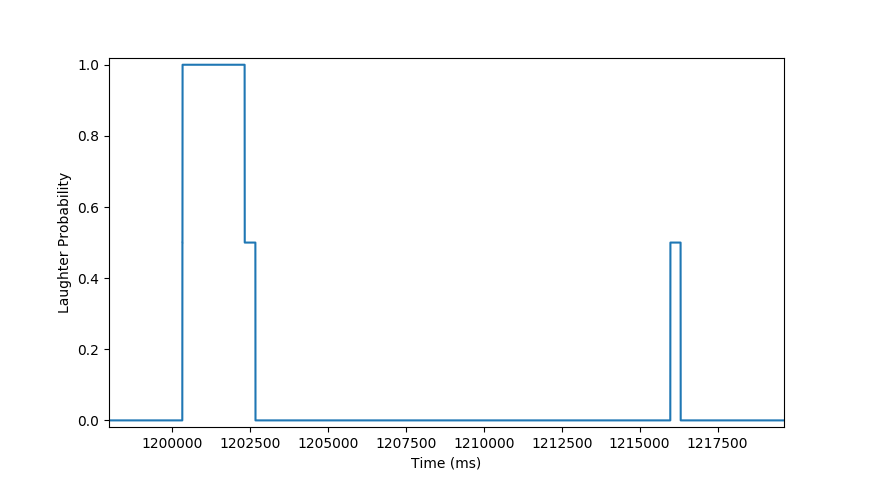
\includegraphics[scale = 0.7]{figs/differences_2.png}
	\caption{In this example, while both classifiers agree that the first laughter instance exists, only one classifier managed to find a second laughter segment.}
	\label{laughter_classification_differences_2}
\end{figure}
The entire dataset used for training the model in this report was only classified by one person, despite the promising results and improvements enabled by multiple classifications. This was due to time constraints, and the inability to convince people to listen and classify 15 hours of speech for no apparent reward. An ideal dataset should have many classifiers, and the classification used for training could be the average of all the individual classifications. This way, a section of audio which only 50\% of people think is laughter, will only be labelled as 50\% laughter, and the sections of audio at the beginning and end of laughter segments will smoothly transition from non-laughter to laughter and back, rather than an abrupt jump.

\subsection{Preprocessing}

% Noise removal and rough volume normalisation.
% White noise removal from redacted segments.
% mfcc extraction.
	% Also talk about delta's and delta-delta's.
% The per-file normalisation of MFCC values.
% The data storage method for speed and size.

There are many different transformations that the original 44kHz wave audio files must undergo before they are suitable to be used as input data for a TensorFlow model. These transformations can be separated into two parts: the preprocessing, and the TensorFlow input pipeline. Pre-processing takes place prior to any other stage, and consists of transforming the audio files into streams of features which are quickly and easily read by TensorFlow. These streams are then further transformed by TensorFlow at training-time into their final form before being used to update node weights. This latter section will be talked about in Section \ref{section:input_pipeline}. There are a few different procedures undertaken in the pre-processing stage, and this part of the pipeline is visualised in Figure \ref{preprocessing_pipeline}.

\begin{figure}[H]
	\centering
	\vspace{0.5cm}
	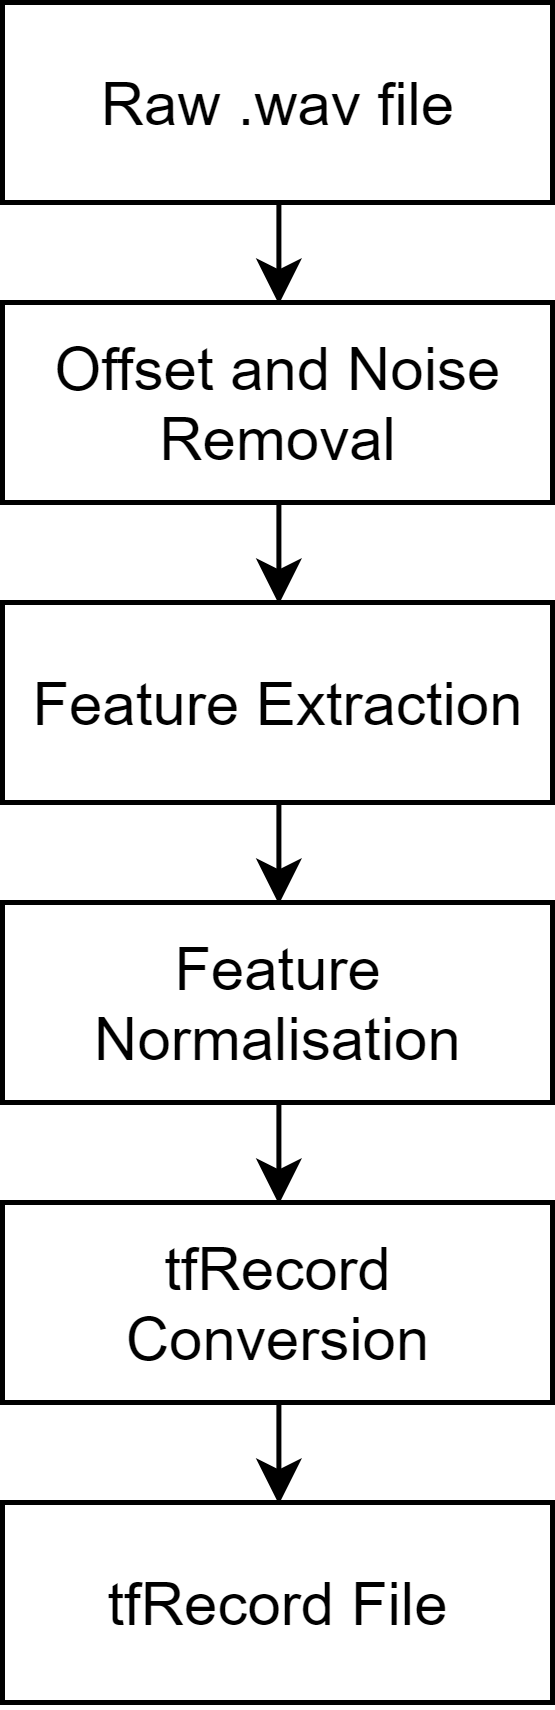
\includegraphics[scale = 0.17]{diagrams/preprocessing.png}
	\caption{The preprocessing pipeline.}
	\label{preprocessing_pipeline}
\end{figure}

\subsubsection{Volume Normalisation and Noise Removal}

Most audio files in the dataset were recorded at different times, on different recording devices and in different locations. In machine learning, it is important to attempt to normalise all the data, and attempt to make it as similar as possible, so the neural network can attempt to learn the subtle differences between what is and isn't laughter, and not let it be affected by the differences in recording equipment or location. Audacity was used for all preprocessing tasks.

\begin{figure}[H]
	\centering
	\vspace{0.5cm}
	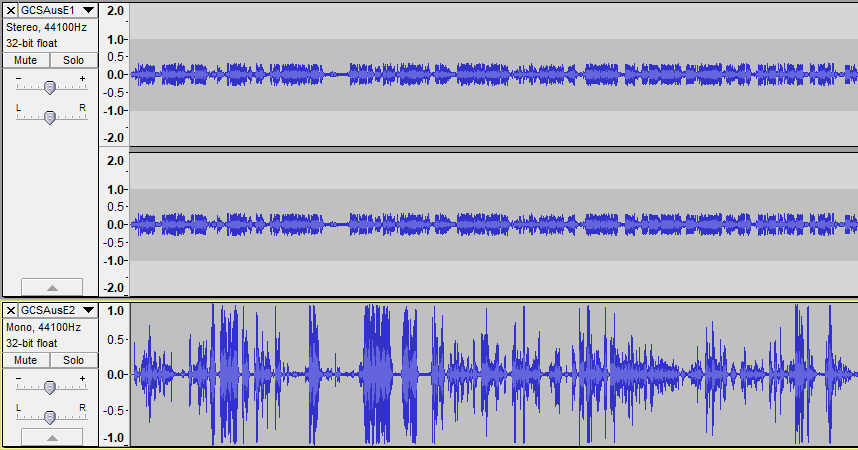
\includegraphics[scale = 0.5]{figs/origional_waveforms.png}
	\caption{The waveforms of two difference audio files before preprocessing. The top recording is in stereo, and much softer than the bottom recording. These are the differences preprocessing attempts to remove.}
	\label{before_preprocessing}
\end{figure}

The volume of each audio file should be roughly equal, because a louder file will produce larger features. This will reduce the ability for the network to determine the actual volume of the audio in the file. The `Amplify' function in Audacity was used to boost the volume of quiet files until they were roughly the same volume. This is not a precise method of normalizing the volume between different files, but the majority of this volume normalisation will be taken care of in the file-by-file feature normalization later, so it isn't important that this volume normalization is incredibly precise, only that each file sounds roughly the same.\\
\\
Next, due to the nature of this dataset, several audio files were recorded in noisy environments and had large amounts of noise distorting the audio. In this section `noise' refers to the repetitive drone of machines, electronic sinusoidal noise, and artefacts of the recording device. These types of noise are largely sinusoidal, and overlay the audio throughout the entire clip. Due to the repetitive nature of this noise, it is effectively filtered out by Audacity's `Noise Reduction' filter.\footnote{For more information on the specifics of this function, an explanation of how the algorithm works can be found here: \url{http://wiki.audacityteam.org/wiki/How_Audacity_Noise_Reduction_Works#algorithm}} This filter takes a sample of a section of the original audio file which contains only noise and no additional sounds. It takes the Fourier Transform to create a noise profile, and specifically attenuates these frequencies. This method was used to reduce the amount of noise in the original audio files, as constant sound at a certain frequency will distort to values of the features extracted from the audio.\\
\\
Lastly, the original dataset audio contained sensitive information about many locations and people who were the subject of conversation. Any names or locations have been removed from the dataset, however they have been replaced by a harsh white-noise sound. Just as other distortions will, these segments of white noise will also reduce the accuracy of the laughter detector.  Audacity was used to remove as many of these segments as possible.

\subsubsection{Feature Extraction and Normalisation}

After roughly normalizing the volume and removing noise, features need to be extracted from the audio waveform. This is a technique common to almost all speech recognition systems, and is of fundamental importance. From the book: ``Fundamentals of Speech Recognition'', it is said that: ``... perhaps the greatest common denominator of all recognition systems is the signal-processing front end, which converts the speech waveform to some type of parametric representation (generally as a considerable lower information rate) for further analysis and processing.''\cite{rabiner1993fundamentals} The book goes on to dedicate an entire chapter to discussing and comparing the various different methods of signal processing used to extract series of features for the data input to a speech recognition system. As alluded to in that quote, this is especially important as it reduces the rate of information needed to be processed by the neural network. In another publication by world leading researchers: ``This non-adaptive but highly engineered preprocessing of the waveform is designed to discard the large amount of information in waveforms that is considered to be irrelevant for discrimination and to express the remaining information in a form that facilitates discrimination...''.\cite{hinton2012deep} For example: over a single second of audio, lets assume that a handful of syllables are pronounced by the speaker. All information in the time series waveform is not necessarily needed to understand which syllables were said. Rather than the 44000 floats used to describe the waveform over one second, signal processing techniques can be used to extract the amounts of different frequency sounds from the audio. This 44000 floats/second waveform can be reduced to roughly 1000 floats/second of extracted features. This is greater than an order of magnitude size reduction, while only losing a fraction of the audio information. This allows researchers to train networks on much larger datasets, for much longer than would be possible if the entire waveform were to be used.\\
\\
While there are many different feature extraction methods, the features used for laughter detection were chosen to be Mel Frequency Cepstral Coefficients (MFCC's). MFCC's are essentially filter banks, measuring the intensity of audio at different frequencies. The frequency bins are scaled to immitate the ranges of audio humans hear at, and the intensity is logarithmically scaled to further imitate the scale of the human ear. MFCC's were chosen because they have been used recently in a number of leading speech recognition systems.\cite{mozilladeepspeech} The number of MFCC features to generate is variable, and is generally between 12 and 26. 20 MFCC features were used in this system.\\
\\
Another feature commonly included in neural networks learning from MFCC's are their deltas and delta deltas. Training a network on MFCC's allows it to attempt to make a classification based on a snapshot of time. Deltas are the first derivative of the MFCC features, and delta deltas are the second derivative. Appending these features to the original MFCC features gives the network more information about the way the MFCC's will change in the future. Giving the network more features to train on may result in higher quality discrimination.\\
	% Additional features
	% Spanning features for non-sequential networks.
	% Clip number, feature number, labels
\\
In addition to the features listed above, the file number, sequence number, and laughter labels were appended to the list of features. The laughter labels are a one-hot encoded vector for the two different classifications: laughter, and not laughter. They are used for training in the training set, and purely for plotting against and evaluating accuracy in the test set. The sequence number refers to the nth set of features of the file. The first set of features is number 1 and is generated from the audio starting at 0.00s, and ending at 0.02 seconds. The next sequence is 2 and so on. The clip number is a unique number identifying the specific file the audio sample came from. These last two numbers, the clip and sequence number, are used in the test set when plotting the probability of the output. The clip and time in the clip when laughter occurred can be generated. This is helpful in evaluating which sounds trigger the network to recognise laughter.\\
\\
Next, each feature is normalized on a file-by-file basis. After the MFCC's for an entire file have been generated, the features are normalized accordingly by subtracting the mean of that particular feature, and then dividing by the standard deviation.
\begin{equation}
	x\prime = \frac{x - \bar{x}}{\sigma^2}
\end{equation}
Perhaps the following pseudo-code can help convey what has been done.
\begin{lstlisting}
for each 20ms frame of audio
    generate 20 MFCC's
end
save 2D value as array. Size = [number of 20ms segments, 20]

for x in 1 to 20:
    a[:,x] = (a[:,x] - mean(a[:,x])) / stddev(a[:,x])
end

// Repeat this for each file
\end{lstlisting}
This normalization further helps remove any biases, differences in volume between files, and also centres the values around zero. This is an important property of the input data for any neural network.\cite{lecun2012efficient}

\subsubsection{tfRecord Conversion}\label{section:tfRecord_conversion}

TensorFlow is used in this report to create and train the neural networks to classify laughter. TensorFlow provides a simple Python API to allow the creation of many types of neural networks with relative ease. A much more in depth discussion on TensorFlow and how it is specifically used to read data and train networks will take place in Section \ref{section:Tensorflow}, but this one important part of preprocessing occurs separate to the whole TensorFlow pipeline, and is crucial to running an efficient training pipeline.\\
\\
At this point in the pre-processing pipeline, data is saved in a two dimensional array of size: [number of frames, number of features]. A primitive method of saving this array for use by TensorFlow would be to use a comma separated variable file (CSV). This saves all numbers and variables as UTF16 variables. This is human-readable and neat, but very computationally inefficient. To read any single set of features from the table, the entire line must be parsed by a CSV reader, stacked into a Tensor, and parsed to the next stage of the input pipeline. This is orders of magnitude slower than reading a binary file, and if more complex reading is needed, column by column for example, CSV files become even more inefficient. Google recognised this when creating TensorFlow and created a custom binary data type called tfRecords which can be used for data storage.\\
\\
TfRecords have the ability to store many different data types in the same file as a sequence of binary strings. It is similar to HDF5 (Hierarchical Data Format) which is designed to store and organise large amounts of data efficiently, but with a few extra features built in. TfRecords contain sets of key-value `features' where the key, (a string) maps to binary data which can be many different data types. Reading this data is fast, and the hierarchical format leads itself to being organised into Tensors quickly and efficiently.\\
\\
Consequently, the final stage of the preprocessing pipeline is to convert every audio file's set of features into a tfRecord file for fast accessing by TensorFlow. Adding this step increased the training speed of the network by an order of magnitude and simultaneously reduced the file size by $\sim$20\%.

\subsection{Initial Analysis}

Before taking the large laughter database straight to TensorFlow, it is useful to attempt to visualise differences in our features before trying anything more complex. For example, if we can show that laughter is easily separable just by observing feature values, why bother going to all the trouble using neural networks if this problem can be solved another way. In reality, it is expected that there will be no simple way to discriminate between laughter and non-laughter, because if there way, problems like speech detection would have been solved a long time ago. It is still useful however, as it will give a `feel' for the data, which may help when building a more complex network.\\
\\
Simply looking at the audio waveform for examples of audio and laughter is a good place to start.

\begin{figure}[H]
	\centering
	\vspace{0.5cm}
	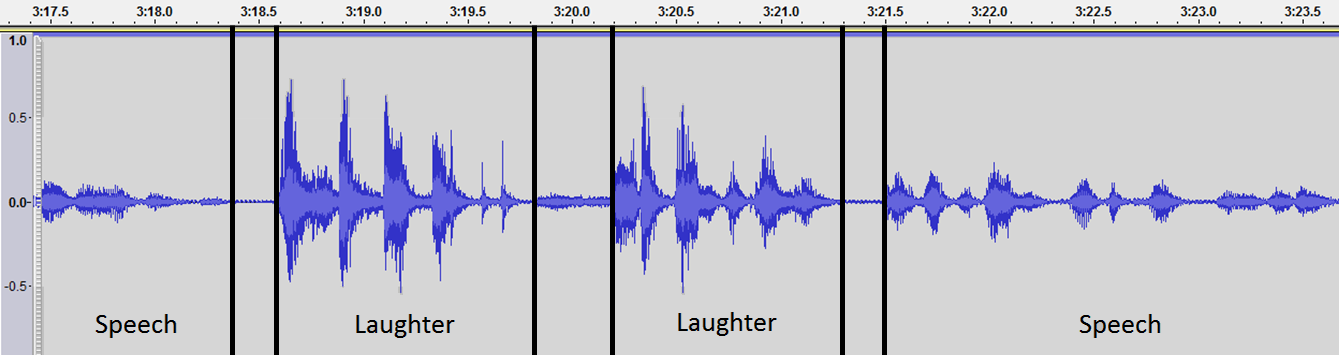
\includegraphics[scale = 0.4]{figs/time-series2.png}
	\caption{The time series waveform of an audio sample containing both laughter and speech.}
	\label{time-series2}
\end{figure}

\begin{figure}[H]
	\centering
	\vspace{0.5cm}
	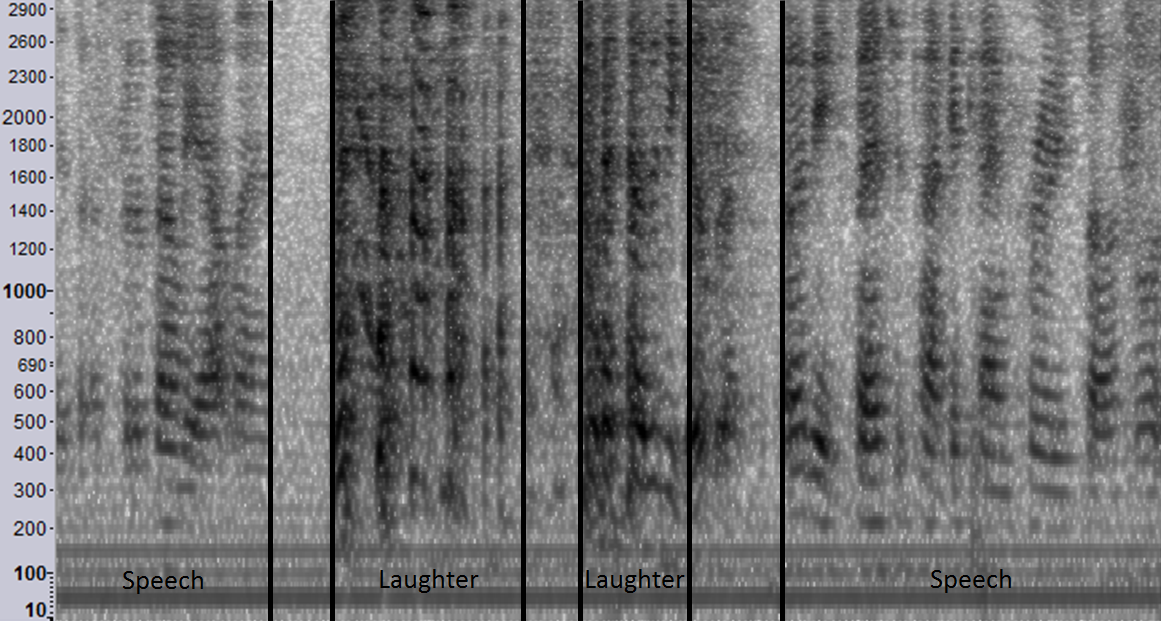
\includegraphics[scale = 0.462]{figs/spectrum2.png}
	\caption{A spectrogram visualisation of the same waveform shown in Figure \ref{time-series2}.}
	\label{spectrum2}
\end{figure}

The waveforms shown in Figure \ref{time-series2} and Figure \ref{spectrum2} both show the waveforms of laughter and speech in different ways. There are differences between them visually in both representations, but there are no defining features of either one. In the time series waveform, the laughter appears to be louder than surrounding speech, and in the spectrogram visualisation, the finer harmonic details in speech appear to be lost, or at least much more complicated in laughter. Either way, this audio sample is interesting and shows some differences, however the dramatic differences in laughter can actually sound like make this a significantly harder problem. Laughter is not always louder than speech however, so creating a system that purely recognises volume would miss classify loud speech and soft laughter.\\
\\
These waveforms convey some different features, however any network trained on this dataset isn't trained on the full waveform data used to generate these pictures. All neural networks will be trained on normalised MFCC features. In order to visualize this, lets plot that same section of audio again, but this time look at the normalised MFCC features.

\begin{figure}[H]
	\centering
	\vspace{0.5cm}
	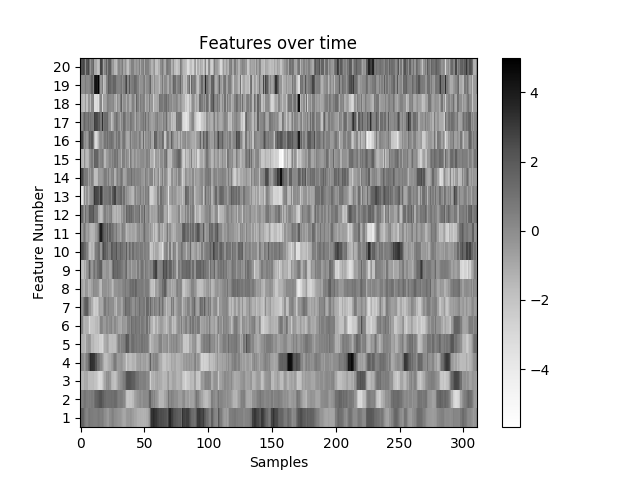
\includegraphics[scale = 0.8]{figs/features_visualisation_grey.png}
	\caption{The same 6 seconds of audio as Figure \ref{time-series2}, and Figure \ref{spectrum2}, but in MFCC feature form.}
	\label{mfcc-visualisation}
\end{figure}

% This is performing PCA and t-SNE on the origional data and features.
Talk about t-SNE and PCA and whatever else here.

\begin{figure}[H]
	\centering
	\vspace{0.5cm}
	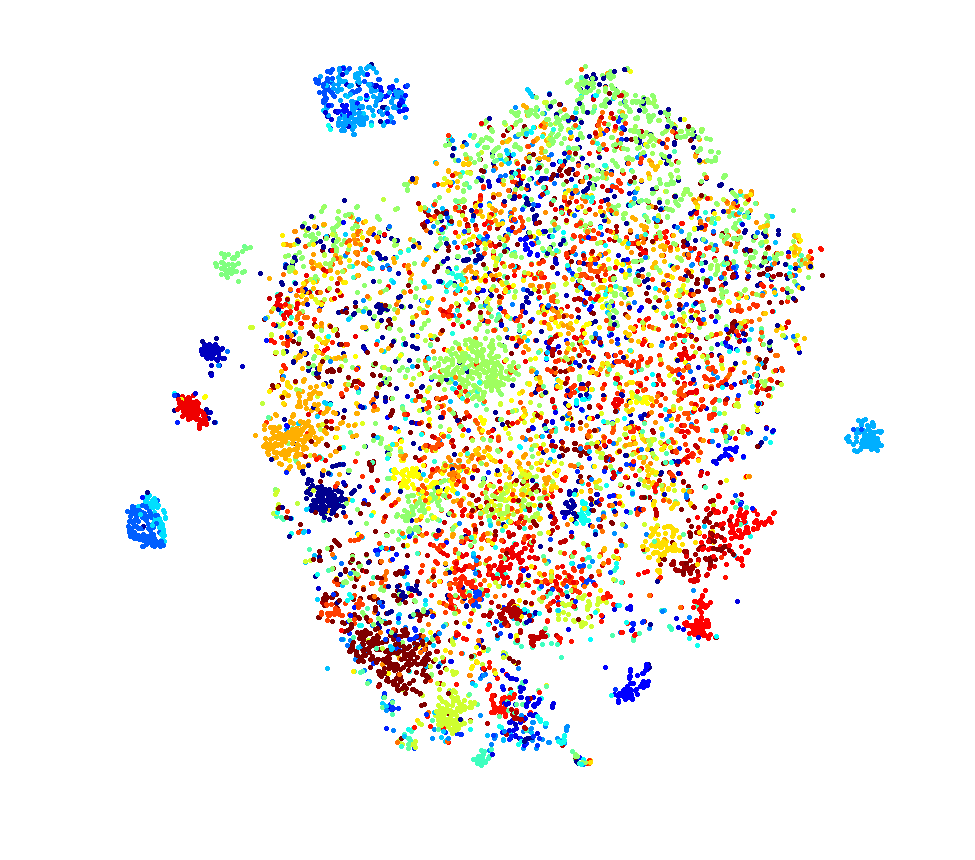
\includegraphics[scale = 0.5]{figs/tsne2.png}
	\caption{t-SNE plot of a randomly selected set of frames of features from un-normalized MFCC's.}
	\label{tsne1}
\end{figure}

% Show that the data doesn't really appear to be especially seperable.

% Matlab Neural networks.


\subsection{TensorFlow}\label{section:Tensorflow}

% What tensorflow is, and why I chose to use it over something like MATLAB.

TensorFlow is an open source software library which allows programmers to implement complex machine learning algorithms with relative ease. TensorFlow contains functions to perform efficient n-dimensional matrix (tensor) manipulating and calculation, by building a graph of mathematical functions which the tensors `flow' between. By generalizing these operations to nodes of the graph, general gradient calculation for back propagation through neural networks can be done with a single function, allowing any confident programmer to fiddle with these networks and use them to train intelligent systems on almost anything. It also supports many other complex features such as: deployment on mobile devices, GPU acceleration, and scalable distributed training and testing across multi CPU/GPU systems. Since it is open source, it also features complex and state of the art systems contributed by leading researchers in their fields\\
\\
TensorFlow was chosen as the program to be used in this project, over other competing programs such as MATLAB's neural network toolbox, scikit-learn, Caffe, and many others, because of its lower level implementation and the finer control it provides. In addition to this, it is open source, has copious documentation, and will allow the quick and effortless prototyping of many different types of neural networks with different parameters. TensorFlow is also packaged with TensorBoard, a network visualisation tool, allowing the network architect to visualise the network's node weights, accuracy, cost, and any other feature instantly and effortlessly. Initially MATLAB's neural network toolbox was trialled, however it lacked the basic functionality to support datasets larger than the total amount of memory available to the system. This would have made training the laughter detector impossible, so the switch was made to TensorFlow immediately.

\subsubsection{Input Pipeline}\label{section:input_pipeline}

% Talk about the many different input pipelines I've tried but mainly:
	% The frame by frame batches
	% The sequences of frames batches.
	% Remember to insert pictures of the networks from tensorboard.

\begin{figure}[H]
	\centering
	\vspace{0.5cm}
	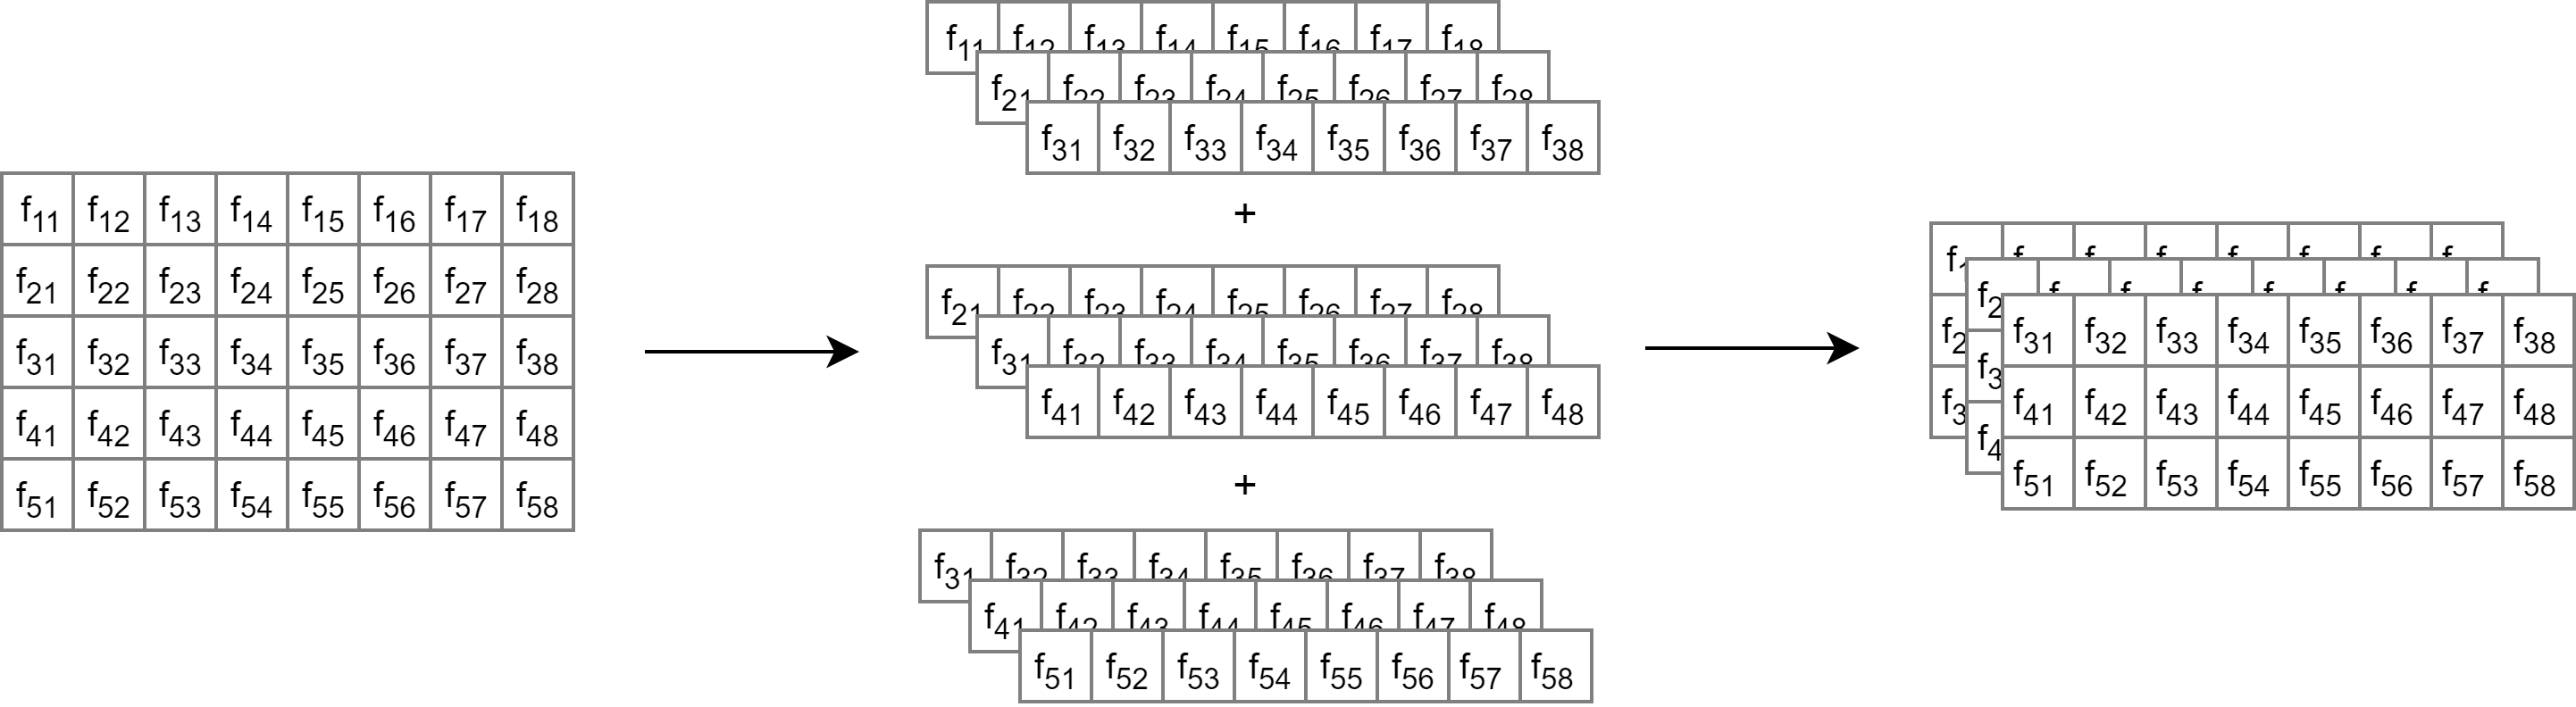
\includegraphics[scale = 0.15]{diagrams/sequence_generation.png}
	\caption{A diagram showing a visual representation of the mapping used to generate sequences for a neural network expecting sequences. The original format on the left is two dimensional, with the different features along the x axis, and the different frames along the Y. This is transformed into the three dimensional tensor on the right, with features on the X axis, different sequences on the Y axis, and the frames which make the sequences on the Z axis.}
	\label{sequence_generation_mapping}
\end{figure}

\subsubsection{Models}

% Talk about all the various TensorFlow models I attempted to use.
	% mlp
	% sequence mlp
	% ltsm
% Talk about additional features of the networks
	% Dropout
	% Batch normalisation
	% Shuffling
	% Activiation Function
		% Relu clipping


\subsubsection{Cost Function}

% Talk about the cost function I used. Maybe put this in the previous section or something.

\subsubsection{Initialization}

% Talk about initialization of the network.
	% Xavier Initialisation

\subsubsection{Hyper parameters}

% Show results of big tests of many different networks to find best hyper params.

\subsubsection{Training}

% Talk about my training methods and how I split data and train on it.
% Not so much because it's interesting or unique, but to show I did it correctly.

\subsubsection{Model Evaluation Metrics}

% Talk about accuracy and sensitivity and specificity.
	% Talk about all the different metrics and how I should use these to actually measure 'goodness' of the system
% Also talk about the creation of the pictures I do of the network every time I finish training.
	% The ROC curve
	% The audio probability graphs
	% The Confusion matrixes.

\newpage

\section{Results}

% Talk about the metrics of the best network I made.

\section{Discussion}

% Maybe the in depth results will take place in this section, and not above.
% Talk about funky things that my networks have picked up. All the weird things.
% Different features of the audio my system is picking up.

\subsection{Improvements and Future Study}

% Talk about the myriad of features I'm sure I will have wished I could get around to, and would love to see the results of, but didn't quite have enough time to do.
% If someone else were to do this thesis, the things I would have liked them to do are:
	% Different types of laughs: genuine vs polite

\section{Conclusion}

% Conclude. Another brief summary of everything I have done, and close.

\newpage

\bibliography{report}
\bibliographystyle{IEEEtran}

\end{document}
